\subsection*{Abstract Syntax Tree}\label{sec:AST}
The parser creates a parse tree which contains a node for each production of \gls{gamble}'s grammar.
This tree contains unnecessary information, which makes it difficult to traverse the tree and check for the semantics of \gls{gamble}.
Therefore the tree will be transformed into what is known as an \acrfull{ast}.
An \acrshort{ast} should be able to express the same source code as the parse tree.

The compiler developed by the project group implements a pretty printer.
A pretty printer is used to ensure that no information is lost in the process of converting the source code into a parse tree followed by the conversion to an \acrshort{ast}.
It does so by traversing the \acrshort{ast} and outputting the original source code from the information gathered by the traversal, except for code which is not parsed, e.g. whitespace and comments.
This output should then be a valid input for the compiler and also result in an identical program, apart from whitespaces and comments.
If this holds true not only does it serve to prove that the pretty printer is working as intended, but also that no information is lost from the \acrshort{ast} transformation.
\todo[inline]{Dette prettyprinter er noget sjovt placeret. MP - Sýnes nu det er meget fint, vi nævner at man skal kunne lave en pretty printer lige inden, så bør vi vel også forklare hvad det er :) ? - Søren - Jeg har slettet at det er nævnt lige inden eftersom det der stod allerede står i PP afsnittet hvor det er indledt med en forklaring om det - Marc}
A transformation from a parse tree to an \acrshort{ast}, on the declaration: \texttt{int a = 5;} using the grammar of \gls{gamble} can be seen on \myref{image:AST}

\begin{figure}
		\centering
	 	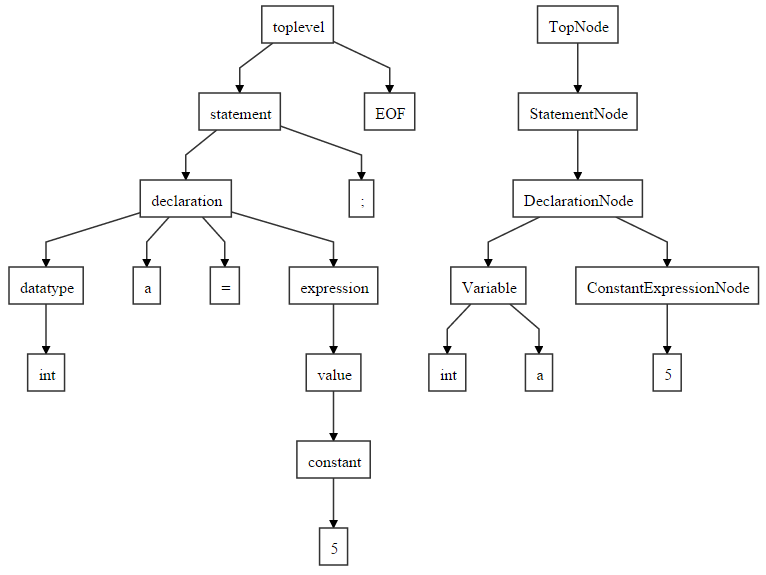
\includegraphics[width=0.8\linewidth]{figures/Trees/AST.PNG}
		\caption{The tree on the left is the parse tree, and the tree on the right is the AST, which still contains all the information from the parse tree.}\label{image:AST}
\end{figure}

The parse tree is generated using a parser produced by providing ANTLR with a grammar, which means that ANTLR decides which information is contained on the nodes of the tree.
The nodes of the \acrshort{ast} can therefore be made to contain information for type and scope checking, which helps in the contextual analysis phase.\todo{det er lidt usammenhængende med det førnævnte, det er vel ikke som et resultat af at ANTLR laver parse træet, at AST'et KAN holde på type og scope check info? - Marc}
To make this transformation the following is needed: classes for all the nodes of the \acrshort{ast}, a way to traverse the parse tree while using the traversal to create instances of the \acrshort{ast} nodes and binding them together to create a structured \acrshort{ast}.



